% FigureR1_information_flow
\begin{figure}[H]
\centering
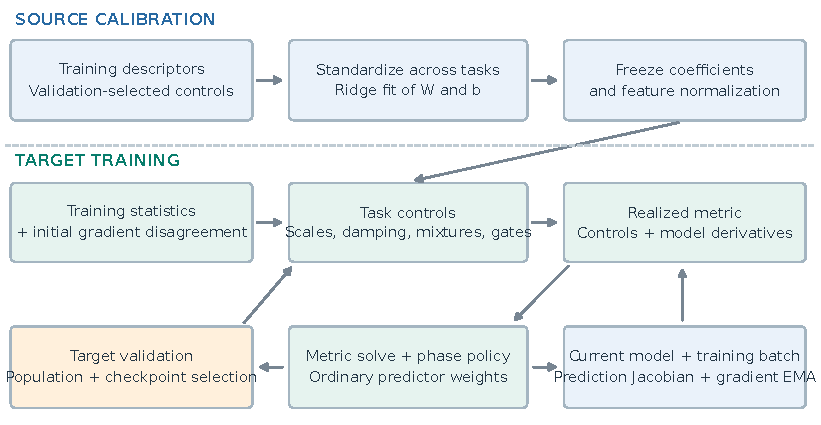
\includegraphics[width=\linewidth]{figures/FigureR1_information_flow.pdf}
\caption{\rev{Information flow in the task-conditioned controller.} Source validation selects controls used to fit the initializer. On a target task, descriptors initialize controls, current model derivatives form the metric, and target validation selects population updates and checkpoints. Test targets enter only final evaluation.}
\label{fig:source-flow}
\end{figure}

% FigureR2_control_and_cost
\begin{figure}[t]
\centering
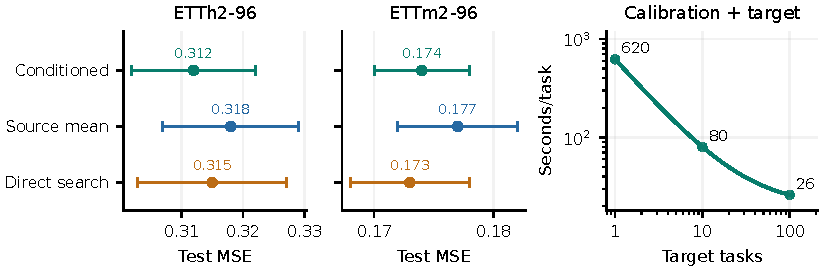
\includegraphics[width=\linewidth]{figures/FigureR2_control_and_cost.pdf}
\caption{\rev{Task initialization and calibration cost.} Left/middle: test MSE with seed standard deviations. Right: source-calibration plus target-adaptation cost per task, $600/N+20$ seconds; loading, descriptors, and final reporting are excluded from this subtotal. All arms use the same target cap and validation opportunities.}
\label{fig:direct-search}
\end{figure}

% FigureR3_dlinear_convergence
\begin{figure}[t]
\centering
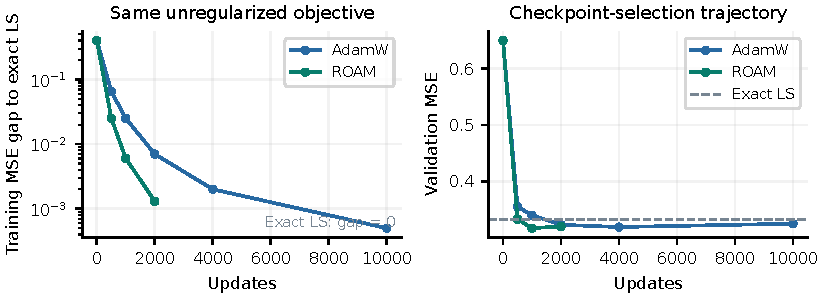
\includegraphics[width=\linewidth]{figures/FigureR3_dlinear_convergence.pdf}
\caption{\rev{DLinear convergence and validation behavior on ETTh2-96.} Left: full-training MSE above the exact unregularized minimum; right: validation trajectories. Lines connect recorded evaluations. The training optimum and validation-selected checkpoint are different objects; the update allocations do not imply equal wall-clock cost.}
\label{fig:convex-control}
\end{figure}

% FigureR4_phase_policy
\begin{figure}[ht]
\centering
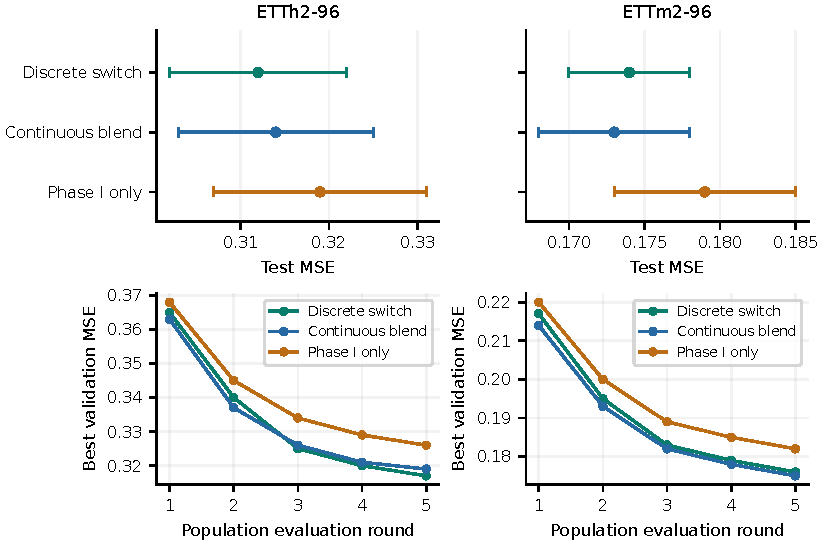
\includegraphics[width=\linewidth]{figures/FigureR4_phase_policy.pdf}
\caption{\rev{Phase policy and validation behavior.} Top: final test MSE and seed standard deviations. Bottom: best validation MSE by population evaluation round. Round indices denote evaluation opportunities, not exact elapsed times.}
\label{fig:phase-comparison}
\end{figure}

% FigureR5_classification
\begin{figure}[ht]
\centering
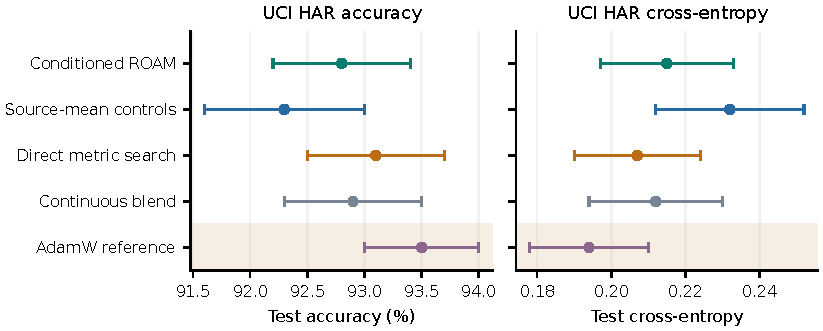
\includegraphics[width=\linewidth]{figures/FigureR5_classification.pdf}
\caption{\rev{Loss-interface extension to temporal classification.} Error bars show seed standard deviations. The shaded AdamW row has a separate update allocation; source-calibration cost is separate from each population target cap.}
\label{fig:classification}
\end{figure}

% FigureR6_curvature_diagnostic
\begin{figure}[t]
\centering
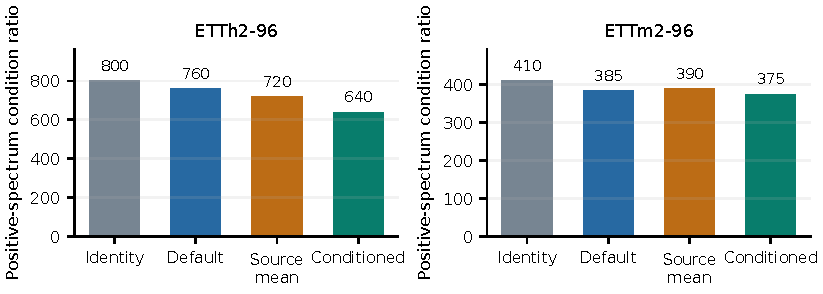
\includegraphics[width=\linewidth]{figures/FigureR6_curvature_diagnostic.pdf}
\caption{\rev{Positive-spectrum conditioning at initialization.} \rev{Means over ten seeds.} Within each seed, metrics share the model state and estimation batch; ratios use the exact full-training Hessian. Flat directions remain outside the positive-spectrum ratio.}
\label{fig:curvature}
\end{figure}

% FigureR7_factorial
\begin{figure}[ht]
\centering
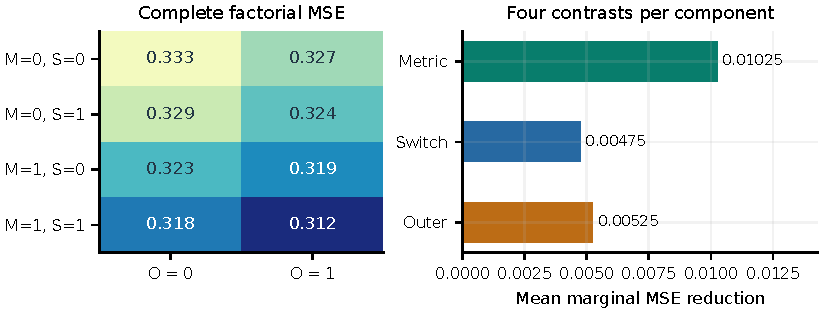
\includegraphics[width=\linewidth]{figures/FigureR7_factorial.pdf}
\caption{\rev{Complete component factorial and descriptive marginal effects.} The left panel uses Table~\ref{tab:factorial}; each right-panel value averages four on/off contrasts. The effects need not sum to the full-system improvement.}
\label{fig:factorial}
\end{figure}

% Figure6_Table20_consistent
\begin{figure}[H]
\centering
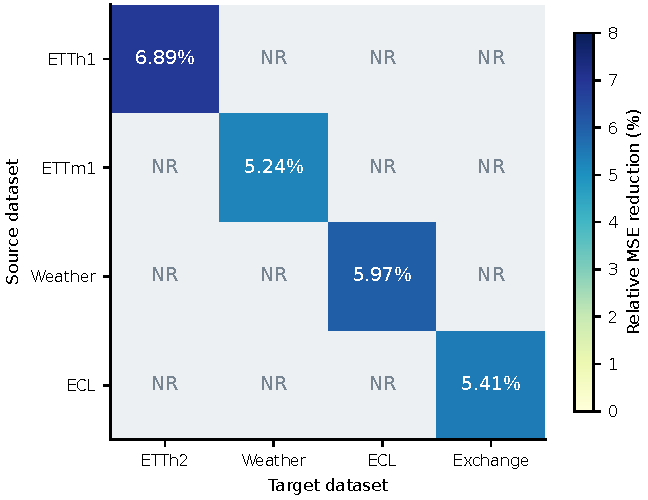
\includegraphics[width=.80\linewidth]{figures/Figure6_Table20_consistent.pdf}
\caption{\rev{Transfer gains reconstructed from the four documented pairs} in Table~\ref{tab:transfer}. Each cell is $100(1-\mathrm{MSE}_{R}/\mathrm{MSE}_{B})$ using the displayed values. NR denotes pairs not individually reported; it is not zero performance change. The 12-transfer aggregate is a separate summary.}
\label{fig:transfer}
\end{figure}

% Figure8_Table15_consistent
\begin{figure}[H]
\centering
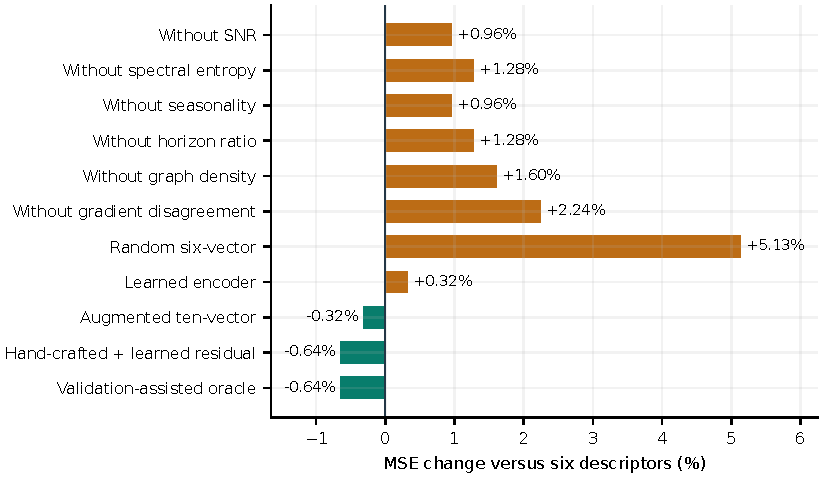
\includegraphics[width=\linewidth]{figures/Figure8_Table15_consistent.pdf}
\caption{\rev{Descriptor effects on a common aggregation basis.} Each bar is $100(\mathrm{MSE}/.312-1)$ from Table~\ref{tab:descriptors}. Positive values denote deterioration; the oracle uses validation-assisted controls. Percentages inherit the rounding of the tabulated MSEs.}
\label{fig:descriptor-ablation}
\end{figure}
